\section{Self-Adaptive Systems (SAS)}  \label{sec:bgSAS}

That are several different ways in which the term \textit{self-adaptation} is defined in literature. Danny Weyns, in his organized tour through the topic of Self-adaptation \cite{EngSAS2018}, attmepts to round up a definition by introducing two complementary principles. 

First, the external principle outlines that self-adaptive systems need to handle autonomously changes, uncertainty, the system's goals and itself. It matches definitions as found in Cheng et al. \cite{SASResearchRoad2009}, which characterizes it as the system's ability to "adjust their behaviour in response to their perception of the environment and the system itself". 

Second, the external principle says that the domain concerns of the system need to be separated from its adaptation concerns, in different parts or modules. This principle distinguishes self-adaptation from other adaptation techniques, like exceptions in programming languages for instance, and comprises definitions that consider the usage of closed feedback loops, like the one from Garlan et al. \cite{RainbowSASMapek2004}.

Weyns, in the same work \cite{EngSAS2018}, also provides a conceptual model of a self-adaptive system that complies with the two principles mentioned. Figure \ref{fig:SASConcepModel} displays the model, which is composed of four basic elements: a managed system, a managing system, the adaptation goals and the environment.

\begin{figure}[!h]
	\centering
	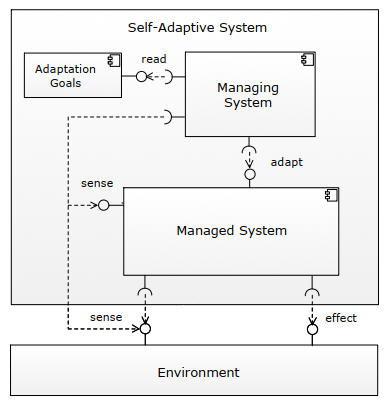
\includegraphics[width=0.5\textwidth, keepaspectratio]{img/SAS_conceptual_model.png}
	\caption{Conceptual model of a self-adaptive system~\cite{EngSAS2018}}
	\label{fig:SASConcepModel}
\end{figure}

\begin{itemize}
    \item \textbf{Managed System:} is the module responsible for the concerns of the application domain. It runs the software that produces the system's expected result and that executes the adaptation plan proposed by the Managing System. It is capable of sensing the environment and causing some effect to it.
    
	\item \textbf{Managing System:} Module whose main goal is to manage the managed system. This is done by monitoring the states of the managed system and the environment and coming up with an adaptation plan in order to fulfill the goals stored in the Adaptation Goals module. Weyns and Iftikhar \cite{Weyns2016ModelBasedSA} further detail this component by specifying its realization through a MAPE-K based feedback loop	\cite{mapek2003}, which comprises a Monitor, Analyze, Plan and Execute modules that partake common knowledge.
	
	\item \textbf{Adaptation Goals:} Refers to the concerns of the managing system that usually depict the software qualities of the managed system. They can be differentiated by four main principles: self-healing, self-protection, self-configuration and self-optimization \cite{mapek2003}.
	
	\item \textbf{Environment:} Physical or virtual entities from the external world that interact with the system and are not controlled, or managed, by it.
    
\end{itemize}

\subsection{Contexts} \label{sec:context}

A possible definition of context is "any information that can be used to characterize the situation of an entity" \cite{2001DeyContext}. When correctly applied, it allows for a better system development, since it helps to identify the set of actions and characteristics that need to be present so that the requirements are met.

This notion fits in nicely in the field of Self-adaptive systems. This happens because it is tightly related to both the adaptation goals and the environment in which the system operates \cite{2010AliCGM}. On the one hand, it is responsible for changing the stakeholder's goals and the strategies used to satisfy them, as well as quality aspects, based on its characteristics on a certain moment. On the other hand, it is considered the reification of the environment, for it makes the system's surroundings tangible so that the system may sense and effect it.

Another relevant characteristic of contexts is that they only represent partial views of the world \cite{2010AliCGM}. This happens because the system observes the environment not as an end itself, but as a means to fulfill a specific purpose. As an example, a health monitoring system might not see value in the context "the sensor node has a squared shape", but should be very interested in verify that "the sensor is far away from the central node". Krogstie et al. \cite{2003KrogstieMCommerce} list several types of context change that facilitate the identification of useful contexts. They are: spatio-temporal, environment, personal, task, social and information contexts.

A context is said to be monitorable if, and only if, there is a formula of facts and monitorable statements that can define it \cite{2010AliCGM}. This formula, also called world predicate formula, is the result of the process of Context analysis, in which high level contexts are refined into formulas of observable facts that support them. This is particularly relevant to the development of SAS since systems can leverage that when sensing the environment. Context information can be operationalized by the usage of sensors, for example, and the formula can be represented by the combination of the different resource states.


\subsection{uncertainty}

Another way to look at self-adaptive systems is as a temporally completed system, with space for configuration variability \cite{2021UncertaintySASHezavehi}. This enables the system to alter its configurations as the conditions change so that it can cope with unforeseen circumstances that are difficult to anticipate in design time. Such circumstances are named uncertainty and are seen by some researchers as \textit{the} motivation for self-adaptation. This lack of deterministic knowledge can lead to the lack of trust in the results, unintended behavior and unexpected failures during the system's lifetime \cite{2010SWEngInUncertainGarlan}.

Uncertainties can come from several sources. Garlan \cite{2010SWEngInUncertainGarlan} provides an unexhaustive list that includes: 
\textit{Humans in the loop}, which happens when the system relies on the proper behavior of humans to work as expected; 
\textit{Learning}, meaning the usage of artificial intelligence in the system's functioning, which depends on past data and assumes statistical regularity; 
\textit{Mobility}, related to the different types of platform on which the system may be run on, and thus the availabity of resources; 
\textit{Cyber-physical systems}, which considers the increasingly complex relations between physical elements and pieces of software and are inherently uncertain; 
and \textit{Rapid evolution}, that relates to the fast pace of change in requirements, technologies, market and regulations.

Another important aspect that is considered in this work is the characterization of uncertainty in three dimensions, which was proposed by Perez-Palacin and Mirandola \cite{2014UncertaintiesinSASPerez}. According to them, uncertainties can be classified in relation to its: Location, Nature and Level.

Firstly, the Location specifies the place in which the uncertainty is manifested within the model. It can happen in the context, in the structure and in the parameters. The context uncertainty refers to the boundaries of the system, or the types of data that should be incorporated or removed from it. The model structural uncertainty relates to how precisely the model's structure captures the segment of the real world that has to be represented. The input parameters uncertainty is associated with the calibration and values of the system's input variables.

Secondly, the Nature dimension divides the uncertainties in two: Epistemic and Aleatory. On the one hand, the Epistemic are uncertainties that happen because of insufficient or inaccurate data, or even  errors in the method used to generate the knowledge from the data. On the other hand, the Aleatory are uncertainties created by randomness of occurrences or intrinsic unpredictability of some components under investigation.

Thirdly, the Level dimension is a scale that ranges from deterministic knowledge to total ignorance on how much knowledge is still lacking for the system to be examined deterministically. The five levels are as described below:


\begin{itemize}
    \item \textbf{Uncertainty of the 0th order:} Lack of uncertainty.
    
	\item \textbf{The first degree of uncertainty:} The system is ignorant about something, although it is aware of it (i.e., known uncertainty).
	
	\item \textbf{The second degree of uncertainty:} Lack of awareness and information. The system is unaware of its ignorance.
	
	\item \textbf{The third degree of uncertainty:} Absence of a method to determine lack of awareness.
	
	\item \textbf{The fourth degree of uncertainty:} The system is not aware of the orders of uncertainty.
    
\end{itemize}

\subsection{Assurances}

The inherent uncertainty and possibility of high context variation permeating self-adaptive systems create the need of evidence to prove that the system is capable of meeting its requirements during its entire lifetime \cite{assurances2017}. This evidence, also known as assurances, can be defined as "the collection, analysis and synthesis of evidence for building arguments which demonstrate that the system satisfies its functional and non-functional requirements during operation". This is specially important for safety-critical systems because of its safety restrictions and strict guidelines.

Formal methods are considered by the state-of-the-art approaches as the most promising way of providing such guarantees  \cite{assurances2017}. Nevertheless, some uncertainties might be faced only during the system's operation, which makes the off-line solutions insufficient. To address this matter, Weyns et al. \cite{2019PerpetualAssurancesWeyns} introduce the concept of perpetual assurances, which consists of a continuous process performed by both humans and the system to derive and incorporate new evidences. To this end, two types of assurance must be consistently updated  \cite{assurances2017}. First, the evidence that concerns the parts of the system that are little affected by uncertainties and, thus, can be acquired by traditional off-line methods. Second, the evidence regarding the modules taht are considerably impacted by uncertainties. This type of assurance should be synthesized during the handling of the uncertainty, at runtime, for each of the several adaptation functions.

The methods that provide the perpetual assurances can be divided in three categories: the human-driven, the system-driven and the hybrid approaches. Next, one sample strategy from each group will be described.

\begin{itemize}
    \item \textbf{Formal Proof:} A human-driven approach that relies on mathematical calculations performed by automatic theorem provers to demonstrate a set of related theorems based on a formal description of a system. It requires from the developer a thorough domain knowledge of the system and a vast mathematical experience, but provides a reliable and unambiguous evidence. 
    
	\item \textbf{Runtime Verification:} A system-driven lightweight procedure that relies on gathering data from an active system to determine whether specific properties are being violated.
	
	\item \textbf{Model Checking:} A hybrid method that verifies if a property is satisfied by checking all the reachable states in the system. It is typically run offline, but can also be applied online, and can both verify properties in the entire system (a high level abstraction) or just in some specific module.
    
\end{itemize}

\section{Goal Oriented Requirements Engineering} \label{sec:bgGORE}

% \cite{Horkoff2019133}
The degree to which a software system satisfies its requirements has a significant impact on its quality \cite{Horkoff2019}. One of the lenses through which these requirements can be seen is the stakeholder goals. Goal-Oriented Requirements Engineering (GORE) approach that follow a goal-oriented perspective and alludes to the usage of goals for every activity of the Requirements Engineering area and aims to acquire and represent systems and software requirements at the intentional level \cite{van_lamsweerde_system_2003}. Weyns points out, as the fourth wave on engineering self-adaptive systems, that goal-driven adaptation "puts the focus on key elements for the concrete realization of self-adaptive systems” \cite{EngSAS2018}. 
Goal modeling, in particular, reflects what stakeholders hope to accomplish in terms of goals and potential alternate solutions. 

Lamsweerde, in \cite{2001Lamsweerde}, sheds light on the reasons why the Requirement Engineering (RE) field can benefit from a goal-driven perspective. He says that goals offer a precise criterion for requirements completeness and pertinence, which are amongst the main RE concerns. Goals also helps stakeholders understand the reason behind the requirements, since they are easy to grasp by nontechnical decision-makers, they naturally offer the rationale behind them, and they allow for the traceability between the strategic goals and the technical details. Moreover, goals guide the derivation of the requirements that supports them.

The next sections will focus on explaining what is meant by goals, and on detailing a well known framework for goal-oriented contextual modeling and analysis.

\subsection{Goals}

According to the systematic literature review done by ElSayed et al. \cite{ElSayed2017430}, two major definitions of the term \textit{goal} can be found. The first one, introduced by Lamsweerde, says that "goals are objectives achieved by the system through cooperation of agents in the software-to-be and in the environment". While the second one, made by Anton, states that goals are high-level aims that aid in understanding why the system is necessary, and thus, allowing for decisions to be made in accordance to them. 

The formulation of the system's goals specify the properties that need to be assured. In this sense, goals can be crafted depending on the desired level of abstraction. They can reflect high level strategic concerns or low level technicalities \cite{2001Lamsweerde}. Goals also address many sorts of concerns, including both functional and nonfunctional. Functional goals describe goals that are associated with the services to be delivered, whereas nonfunctional goals are related to the system quality. 

Another criterion used to characterize goals divides them based on whether they are quantifiable \cite{ElSayed2017430}. On the one hand, hard goals are the ones that can be formally verified. On the other hand, soft goals cannot have their fulfillment easily determined. The latter allows the comparison of different alternatives of refinement. This distinction is specially useful for the purpose of this work since we are dealing with the provision of assurances to Self-adaptive systems, which is provided through formal methods. Lamsweerde also mentions way of verifying the completeness of the elicited requirements. Let \(R\) be the set of requirements, \(As\) the environment assumptions, \(D\) the domain properties and \(G\) the set of goals. For each goal \(g\), such that \(g \in G\), it must be true that: 

\[R, As, D \vDash g \text{ with } R, As, D \nvDash \text{False}\]

\subsection{Contextual Goal Model (CGM)}

Goal modeling is the technique responsible for representing systems in GORE. As mentioned previously, it provides a powerful way of understanding the needs of the stakeholders besides figuring out the motives behind the development of a piece of software. In the end, a goal model revolves around laying out user goals and ways to meet them \cite{ali_goal_based_2010}. 
This methodology has a major impact in the development self-adaptive systems, which must adapt to different situations like environment changes, system capability changes and changes in the problem to be solved \cite{deloach_capabilities_based_2008}. 

TROPOS \cite{bresciani_tropos_2004} is a software development methodology used to model early requirements. In its heart, there is his modeling language, which is the base for constructing conceptual goal models. It rests in the concepts of actor, goal, plan, resource, dependency, capability and belief. An Actor is an entity that possess intentionality and represents agents, roles or positions. An actor can have none to multiple goals. A Goal is related to the interests of a particular actor, and is divided in soft goals and hard goals, meaning goals whose definition and satisfiability criteria are unclear, for the former, or trenchant, for the latter. A Plan can be defined as "a way of doing something", and as a declaration of which refinement paths should be taken in the directed tree in order to achieve the main goal. A Resource corresponds to an entity with physical or informational attributes. Dependencies are subordination relationships between two actors which point out that one depends on the other, the depender and the dependee, severally. The Capability express an actor's competency to define, choose and execute a plan in order to satisfy a goal. Finally, a Belief declares the world's knowledge of an actor.

A goal model usually utilizes a directed graph tree to delineate the goals in a top-down manner so that goals can be successively refined via AND/OR decomposition and ultimately satisfied by the leaf nodes, which represent tasks that must be performed by actors. On the one hand, AND-refinements tie in a goal with a group of subgoals, and the fulfillment all the subgoals is the only sufficient condition for its fulfillment. On the other hand, the OR-refinement relates a goal to a set of alternative subgoals, meaning that meeting one of the subgoals is enough for satisfying it. The refinement comes to an end when each subgoal is utterly achievable by some particular agent capable of monitoring and controlling it \cite{van_lamsweerde_system_2003}. Figure \ref{fig:andorref} depicts both AND- and OR-Refinements.

\begin{figure*}[!htb]
 \centering
 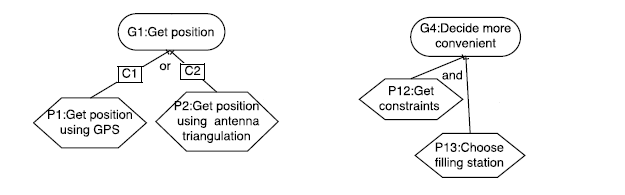
\includegraphics[width=\linewidth]{img/and-or-fill.png}
 \caption{AND/OR-Refinements \cite{Rodrigues:2012}}
\label{fig:andorref}
\end{figure*}  


Since variants were only allowed by regular Goal Models, but not clear-cut defined, an extension of TROPOS, named Contextual Goal Model (CGM), was created to meet the notions of context and goals. It specifies explicitly which changes in the environment can be adopted and when. This allows for systematic derivation of variants based on the  several different contexts that may appear \cite{ali_goal_based_2010}. Figure \ref{fig:andorref} describes \textit{C1} and \textit{C2} as contexts of a OR-refinement, as an example of how contexts are depicted in Contextual Goal Models.

\section{Model Checking} 
% cite 2008 principles of model checking 1.1

\section{Observer Automata} \label{sec:bgobserver}

\subsection{Property Specification Pattern Catalog}


\section{Artificial Immune Systems (AIS)} \label{sec:bgais}

The primary goal of the Biological Immune System (BIS) is to protect the body from potentially harmful material \cite{AISSOA2015}. It is composed by a multilevel defense mechanism that is capable of distinguishing between molecules from the body itself and foreign ones, selecting a specific response to a threat, and enacting an inflammatory reaction in order to maintain the health and safety of the body. All of these activities are capable of evolving through time since they rely on aspects of learning and memory, which are present in the BIS.

In 1986, Farmer et al. \cite{ImmuneSysAdapML1986} sought inspiration in the properties and theories of this biological system to propose a computational model, named Artificial Immune System (AIS). It was built in such a way that the immunological concepts and processes are distilled into algorithms that can be simulated by a computer in order to solve all sorts of problems from the real world. The idea behind it is that, since this system is able to protect us, it might be computationally useful \cite{EvaluateAIS2005}. Nevertheless, by that time, the resources available were not powerful enough to allow its usage in real systems \cite{AdaptiveImmunitySAS2021}.

Recently, the advances in technology enabled complex tasks to be performed in a fast and efficient way. This provided the researchers the tools needed to implement and further improve the application of the immunological concepts into a wide range of problems. For example, AIS techniques have been used in problems like anomaly detection, optimization, classification and clustering \cite{AISSOA2015}. The Negative Selection, along with the Clonal Selection, Immune Network Theory and the Danger Theory are amongst the most researched approaches in the literature \cite{NSAResearch2021}.

This section is structured as follows: initially, the main concepts of the Biological Immune System will be laid out. Then, the Negative Selection algorithm will be explained in depth, for it will be exercised throughout this work.

\subsection{Overview of the Biological Immune System}

As mentioned previously, the Artificial Immune System is a model inspired by its biological counterpart in order to solve computational problems. Therefore, there is a need to introduce the main concepts and processes found in the Biological Immune System so that the analogies and metaphors implemented by the AIS might be better understood. This subsection focuses on providing the reader with the foundational knowledge on the BIS. 

\subsubsection{Main Concepts}

Immunity can be defined as the ability to respond to unknown substances \cite{ICBook2009}. In this sense, the Biological Immune System (BIS) comprises a set of structures and mechanisms which are capable of distinguishing the body's cells from foreign substances and responding adequately. It includes specific organs, cells and molecules. It is a complex, fault-tolerant and distributed multilevel defense mechanism composed of two main layers, namely the innate immunity and the adaptive immunity \cite{Kuby2019}. 

The innate immunity is the body's first line of defense. Inherited from the host's progenitors, it is responsible for a quick or immediate response against infections. It is achieved through physical and chemical barriers or through cellular responses. The barriers are considered nonspecific mechanisms that work as shields against pathogens by blocking them from entering the body. They comprise the skin, mucous membranes on the body's openings and the secretions of both. The low pH of the skin, for instance, inhibits the proliferation and growth of bacteria, while the antimicrobial substances present in saliva and tears keep the antigens from invading through the membranes \cite{ICBook2009}. The cellular response, on the other hand, focus on perceiving the pathogens that were able to surpass the barriers and activating a variety of cellular responses, which include: the ingestion of the substance (phagocytosis), the induction of an inflammatory response and the triggering of the adaptive immunity for a tailor made response. 

The adaptive immunity is an immunological mechanism that is capable of "specifically recognize and selectively eliminate foreign microorganisms and molecules" \cite{ICBook2009}. In contrast with the innate immunity, it has a high level of specificity when dealing with the antigens, meaning that the response is customized and based on the particularities of the foreign substance. The downside is that the response can take days to be performed. Nevertheless, the information from previous infections is persisted in order to achieve a faster response when a similar antigen is detected. In the literature, the adaptive immunity responses is divided into two distinct, but overlapping, categories: the humoral immunity and the cellular immunity.

The first kind of response, called humoral immunity, relies on the interaction between the antigen and B lymphocytes, a specific type of white blood cell also known as B Cell. These cells are created in the bone marrow and, when activated, are able to produce antibodies, which bind to the antigen during the immunological response as a means to destroy it. This can only happen if there is a match between the antibody and the surface of the foreign material. Humans are thought to have \(10^7\) to \(10^8\) different antibodies with distinct chemical compositions \cite{ImmuneSysAdapML1986} that account for the possible variations of antigens that one may find during the course of a lifetime.

The second kind of adaptive response is called cellular immunity and is mediated by lymphocytes called T cells. These cells are also produced in the bone marrow, but are matured in an organ named Thymus. They are responsible for killing tumor cells and cells from the body that were infected by the pathogen (altered self-cells).

\subsubsection{Overview of the Immune Response}

\begin{figure}[!h]
	\centering
	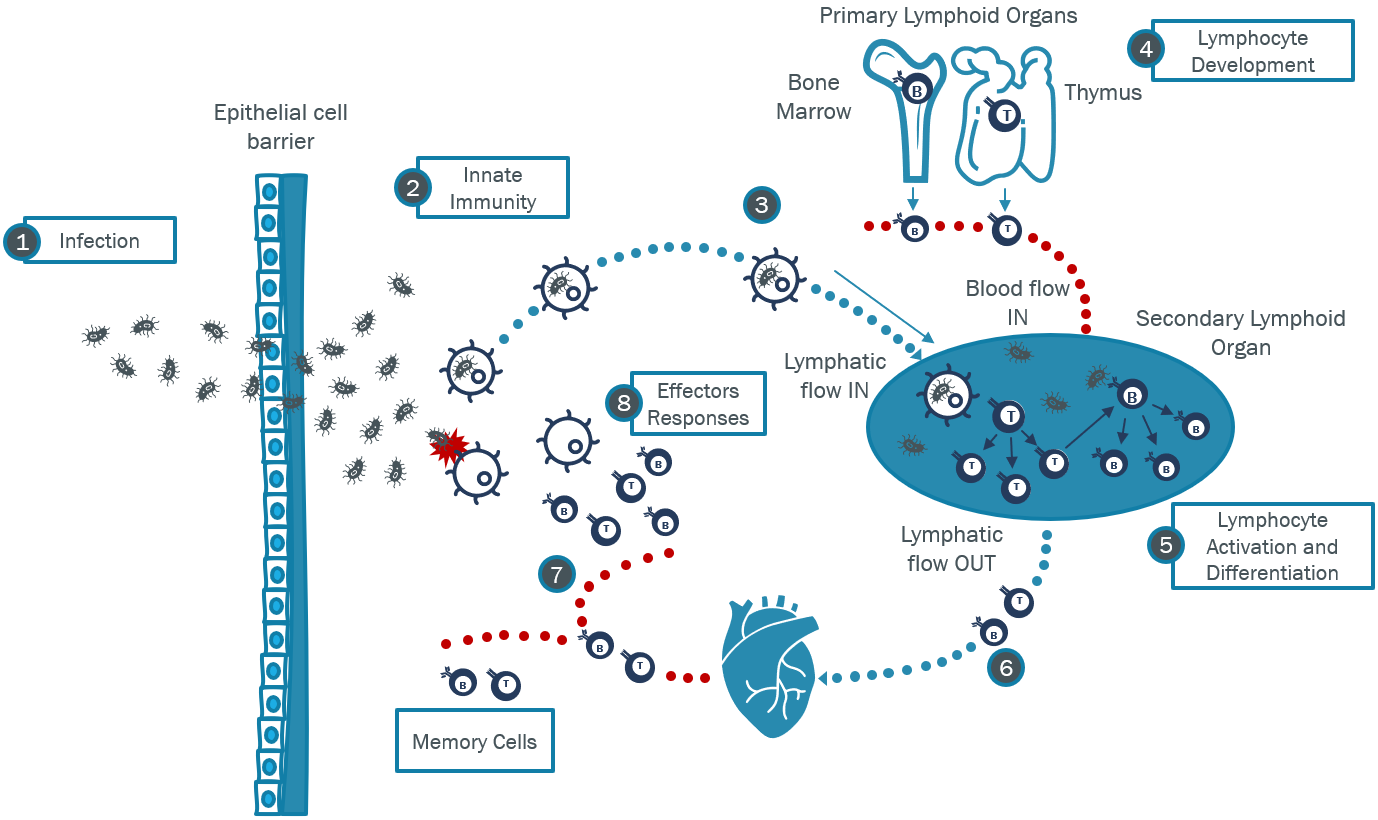
\includegraphics[width=0.9\textwidth, keepaspectratio]{img/overview_bis.png}
	\caption{Main Processes of an Immune Response~\cite{Kuby2019}}
	\label{fig:BISOverview}
\end{figure}

Figure \ref{fig:BISOverview} shows an overview of the main activities that may happen during an immune response. The whole process starts with an infection caused by an antigen that was capable of passing through the physical and chemical barriers of the body (1). After that, when the pathogen is detected by the front line phagocytic cells, a hormone-like protein called cytokine is released by them as to induce a local inflammatory response (2). Besides that, these cells are capable of engulfing the antigen and transporting it through the lymphatic vessels with the objective of enacting the adaptive immune response (3).

In the meanwhile, both B and T lymphocytes are derived in the Bone marrow via a process called hematopoiesis. The receptors of these cells undergo a pseudo-random genetic rearrangement process during their creation that account for the variety of cells, and thus the ability to bind with unseen substances \cite{AIS2014}. While the B cells flow directly through the blood flow into secondary lymphoid organs, the T cells stop at the Thymus to be matured, and then follow the same path as the B cells (4). The maturation of the T cells is a censoring process in which the lymphocytes are tested against proteins of the body. If a T-cell strongly binds to some self-protein, it is discarded. Hence, only the T-cells that did not have a strong bind are allowed to flow through the bloodstream and be used against the pathogen. This process is called Negative Selection and aims at avoiding autoimmune responses.

The adaptive immune response starts at a secondary lymphoid organ, with the arrival of the phagocytic cell carrying the antigen. In this step, a mechanism called Clonal Selection is performed (5). The B and T lymphocytes with a high level of engagement with the pathogen proliferate and mutate (somatic hypermutation) as a means to grow in number and to improve the affinity with the foreign substance. Afterwards, these differentiated cells leave the lymphoid organ and are pumped throughout the circulatory system by the heart (6) until reaching the local of the inflammatory response (7). Finally, the specialized lymphocytes act on the antigens in order to destroy the residual of the invasion (8). These cells are kept as memory cells so that, in the case of a future similar threat, allow for a faster response. 

\subsection{Description of the Negative Selection Algorithm} \label{sec:bgNSA}

One of the fundamental skills of the BIS is the ability to differentiate between the body's own cells and the foreign material. It is called self/nonself discrimination \cite{NSAResearch2021} and helps to protect the body from attacking itself whilst building a strong defense against foreigners. 

As described in the previous subsection, T-cells are created in the bone marrow, where they have their receptors differentiated by a pseudo-random genetic rearrangement process. Later, in the Thymus, they are maturated by being tested with self cells. Lymphocytes that have a strong binding with self cells are discarded, in a censoring fashion. The result of the process is a set of diverse T cells specialized in binding with nonself cells.

In 1994, Forrest et al. introduced an algorithm inspired by this process that is used in the field of change/anomaly detection \cite{Forrest1994}. They have abstracted the concepts of self and nonself so that the process of Negative Selection could be used in more general problems. They have used a file authentication system as an example to instantiate one of the possible applications. In their work, data from legitimate users trying to access a file were thought as the body's own cells, while non-authorized accesses were seen as nonself material, or pathogens. Both types of data were translated into binaty strings, and T-cell detectors were generated as binary strings of the same size which, during the censoring phase, did not match the self data. A change was considered whenever there was a match between some detector and the new data in the monitoring phase.

Since then, even though the main idea of the algorithm was kept, several implementations and adaptations were made to improve its performance and allow for the application it in different scenarios. Dasgupta \cite{NSAResearch2021}, in a recent work, reviewed the literature on this matter and classified the algorithms found based on the following characteristics: data type, data representation, distance function, detector size and initialization.

\begin{itemize}
    \item \textbf{Data Type:} Refers to the type of the data that is used by the algorithm. It can be binary or real value.
    
    \item \textbf{Data Representation:} Related to how the data is structured or formatted. If the data type is binary, it can be shaped as a string or a grid. If it is a real value, the formats are grid and vector. 
    
    \item \textbf{Distance function:} Also called "affinity" or "matching" Function, it is a function that identifies how strong is the bind between the self and nonself data. In the case of binary strings, the most common are the r-chunk, r-continuous bits and hamming distance with its variations. When talking about real valued types, the functions are usually the distance between vectors, like the manhattan, euclidean or minkowski distance. This section will provide more details about this topic latter on.
    
    \item \textbf{Detector Initialization:} Describes how the detectors are generated. In both data types it can be in a random, semi random or adaptive fashion. Further details are provided below.
    
    \item \textbf{Detector Size:} It is usually fixed, but in some real valued algorithms the detectors' size may vary in size in the generation process.
    
\end{itemize}

Some discussion has been made over the Data Type and Representation characteristics since they limit all the others \cite{RevisitingNSA2007} \cite{NSAResearch2021} \cite{ICBook2009}. The advantages of using bit strings are that (1) any data can be presented as a binary string, (2) it facilitates the analysis of the result and (3) categorical data are well represented in this form. Nevertheless, they have a scalability issue that comes with the increased string size. All in all, to achieve the goals of this work, the binary data type and the string representation will suffice.

Even though different implementations may fall in different buckets, Ji and Dasgupta \cite{RevisitingNSA2007} have distilled the three aspects that must be present in an algorithm so that it may be considered a Negative Selection Algorithm. They are:
\begin{enumerate}
    \item The goal is to identify the self-set counterpart.
    \item Change/anomaly detection is performed by using some form of detector. 
    \item The algorithm makes use of only the self-samples during the detector generation.
  \end{enumerate}

The next subsections provide a more in depth view of the algorithm for the binary data type, by showing its overall structure, detailing how the comparisons with the monitored data are made and how the detectors are generated. 


\subsubsection{Algorithm Description} \label{sec:bgNSAOverview}

The Negative Selection Algorithm (NSA) can be divided in two steps: the generation of the detectors, and the actual process of detection of the nonself. These steps are similar to most supervised algorithms, in which there is a training and a test phase \cite{NSAResearch2021}. 

\begin{figure}[!h]
	\centering
	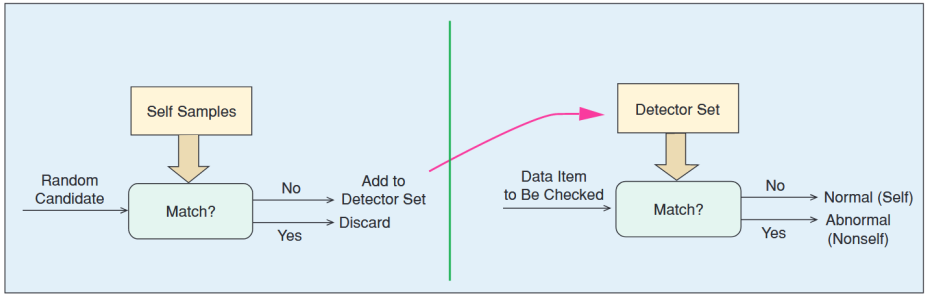
\includegraphics[width=0.9\textwidth, keepaspectratio]{img/NSA.png}
	\caption{The two steps of the NSA~ \cite{NSAResearch2021} }
	\label{fig:NSAOverview}
\end{figure}

Figure \ref{fig:NSAOverview} helps to shed some light on both phases. On the left-hand side, the generation of the detectors is illustrated. In this "training" step, a set of random candidates is generated by some predefined process and undergo a censoring process based on the self samples. The candidates that match the self samples, measured by the distance function, are discarded, while the ones that do not match are added to the nonself detector set. On the right-hand side of the figure, the detection, or "test", phase is shown. The nonself detector set obtained in the first step is tested against the data that is being monitored. The same distance function is utilized here to check whether the new data matches with some of the detectors in the set. In the case of a match, the data is considered abnormal.

For a complete understanding of the inner workings of the algorithm, two important pieces are missing: a description of how the random detector candidates are generated and the definition of the matching function that will account for the affinity measurement.

\subsubsection{Distance Function} \label{sec:bgNSADistance}


First, the Distance function, or matching rule, is an operation that relies on the comparison of characters (or bits) between two strings and provides a score telling how similar (or different) the strings are. Three rules are the most widely used in the literature \cite{EffectBinaryRule2003}: the Hamming Distance, the R-Contiguous and the R-Chunk matching rules. 

% \cite{RevisitingNSA2007}
% a matching rule M can be formally defined as dMx ↔ distance measure between d and x is within a threshold, where d is a detector and x is a data instance.

\begin{itemize}
    \item \textbf{Hamming Distance:} This function measures the number of characters that differ between two strings \cite{ICBook2009}.  Let \(X\) be a string of lenght \(n\) such that \(X = x_1 x_2 x_3...x_n\) and let \(D\) be a dectector with the same lenght, so that \(D = d_1 d_2 d_3...d_n\). The Hamming Distance can be formally defined as:
    \[HD = \sum_i(\overline{x_i \oplus d_i})\]
	 
	where \( \oplus \) is the XOR operation. In this case, a match between \(X\) and \(D\) is said to have happened when the \(HD\) score is below a predefined threshold. Figure \ref{fig:hamm} shows how the comparison is made. The characters at each position are compared and, if they are different, a unit is added to the final score. Therefore, two strigs must have a low score to be considered similar.

	\begin{figure}[!h]
		\centering
		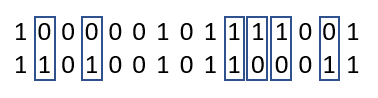
\includegraphics[width=0.4\textwidth, keepaspectratio]{img/hamming.png}
		\caption{Illustration of the Hamming Distance Matching Rule}
		\label{fig:hamm}
	\end{figure}
    
    \item \textbf{R-Contiguous:} Let again \(X\) be a string of lenght \(n\) such that \(X = x_1 x_2 x_3...x_n\) and let \(D\) be a dectector with the same lenght, so that \(D = d_1 d_2 d_3...d_n\). Let also \(r\) be an integer, such that \(0 > r >= n\). This rule defines a match between \(X\) and \(D\) whenever the two strings have at least \(r\) consecutive identical characters starting at any position. This rule was mainly used in the first implementations of the NSA, in which the detectors were created in a generate-and-test fashion \cite{EffectBinaryRule2003}.
    
	\begin{figure}[!h]
		\centering
		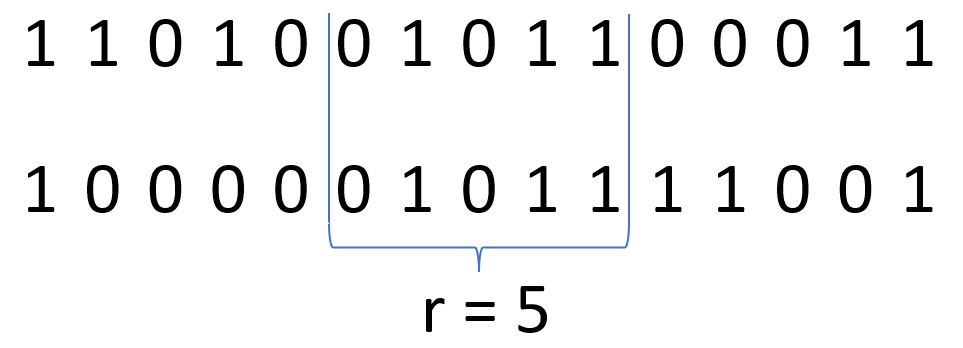
\includegraphics[width=0.4\textwidth, keepaspectratio]{img/rcontiguous.png}
		\caption{Illustration of the R-Contiguous Matching Rule}
		\label{fig:rcont}
	\end{figure}

	Figure \ref{fig:rcont} illustrates this concept. A window of size \(r\) slides searching for a region where the substrings match. If at least one region is found, then \(X\) and \(D\) are considered a match.
    
    \item \textbf{R-Chunk:} Let \(X\) be a string of lenght \(n\) such that \(X = x_1 x_2 x_3...x_n\) and let \(D\) be a dectector of size \(m\) so that \(D = d_1 d_2 d_3...d_m\), with \( m \leq n\). Similarly to the R-Continuous rule, the string and the detector are considered a match if, at a position \(p\), all bits of \(D\) are identical to the bits \(X\) in a window of size \(m\), with \(0 \leq p \leq n - r\).  Hence, the detector is characterized by a chunk of size \(r\) and a starting position \(p\), and can be uniquely identified as \(t_{p, D}\). The practical difference between this rule and the previous one is that this function allows for detectors of any size, which improves the self-space coverage \cite{ICBook2009}.
    
	\begin{figure}[!h]
		\centering
		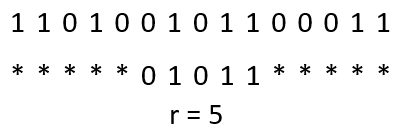
\includegraphics[width=0.4\textwidth, keepaspectratio]{img/rchunk.png}
		\caption{Illustration of the R-Chunk Matching Rule}
		\label{fig:rchunk}
	\end{figure}

	Figure \ref{fig:rchunk} shows an example of this rule. The detector \(t_{6, 01011}\) has size 5 and was a match in the sixth position of the string. The "*" represents irrelevant positions meaning that any character can be matched. 
\end{itemize}

The R-chunk is said to enhance the accuracy and performance of the NSA \cite{EffectBinaryRule2003} because the same generated string can be used as a detector in several positions. Therefore, one can say that lower sized detectors comprise an optimal detector set, since more abnormal data can be detected. Nevertheless, as cited by Wierzchon and Chmielewski \cite{HybridNSA2012}, a study performed by Stibor showed that strings generated with low values of \(r\) are less likely to become detectors. This probability highly increases in the middle range, and is close to 1 for large string sizes. Hence, there is a sweet spot when trying to find the size of the string, which is usually for middle values of \(r\), that aligns accuracy and coverability with efficiency.

\subsubsection{Detector Generation} \label{sec:bgNSADetectors}

% \cite{RevisitingNSA2007}
% On the next level, representation of data space doesn’t define representation of detectors. 

Both Ayara et al. \cite{NSADetectorGen2002} and Dasgupta and Niño \cite{ICBook2009} provide a thorough detailing of the different methods found in literature for the generation of the detectors set for binary data. The most basic approach is the exhaustive detector generation, which was introduced in the original NSA paper \cite{Forrest1994}. The idea is to exhaustively generate random candidates until a big enough set of detectors is achieved. It was reported to be very time-consuming, since the amount of candidates grows exponentially with the size of the self-set \cite{LinearNSA1996}.

\begin{figure}[!h]
	\centering
	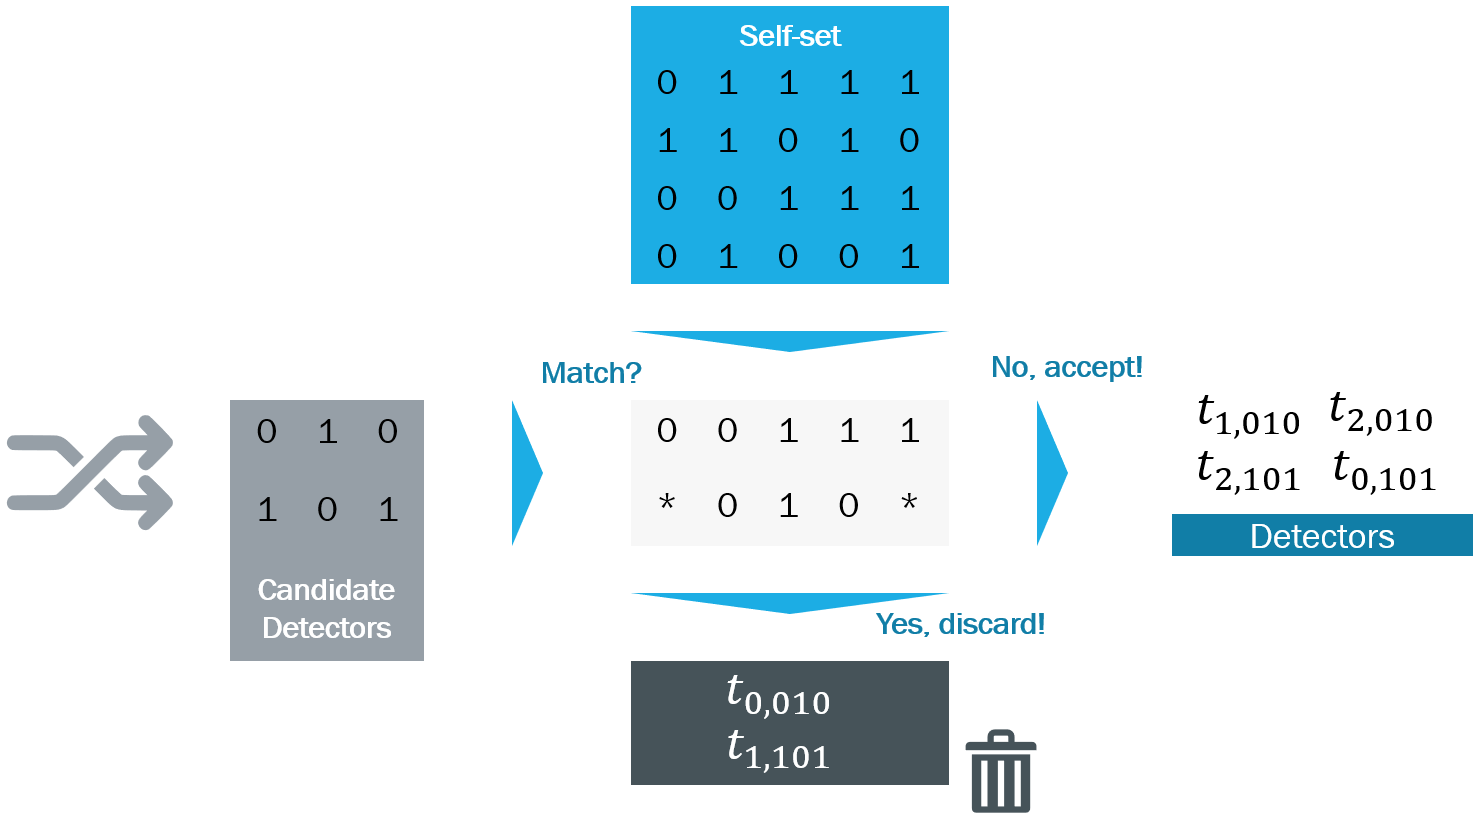
\includegraphics[width=0.6\textwidth, keepaspectratio]{img/exhaustiveNSA.png}
	\caption{Example of the Exhaustive Detector Generation Process~ \cite{LinearNSA1996} }
	\label{fig:ExhDet}
\end{figure}

This generate-and-test method can be further explained with Figure \ref{fig:ExhDet} in which random binary strings are generated and compose the \(R_o\) set. Then, each candidate is tested for a match with the self-set \(S\) by using one of the functions described earlier. In the figure, if the compared strings have at least 2 matching contiguous bits, the candidate is rejected, otherwise it is accepted as a valid detector and joins set \(R\).

The problem with the exhaustive detector generation is that a great number of candidates are rejected during the censoring, making it be inneficient \cite{NSADetGen1996}, besides being costly in terms of computational use of resources \cite{NSADetectorGen2002}. To tackle that, two other approaches arose: the linear and the greedy algorithms, both based on the r-countinuous distance method. 

The linear time algorithm is a two-phase process named after its complexity introduced by D’haeseleer et al. \cite{NSADetGen1996}. Initially, all the strings that are unmatched by the self-set have their recurrence counted. Then, this counting recurrence is used to naturally number the unmatched strings and allow for the picking of random detectors, according to the desired size of the detector's set. Even though this algorithm runs in linear time according to the detector's set and self-set sizes, the recurrence counting requires the storage of all the possible matches two strings can have by using the r-contiguous distance. This means that, although its complexity is linear in terms of time, it is exponential with regard to space. 

The Greedy algorithm is another algorithm introduced by D’haeseleer et al. \cite{NSADetGen1996}, which tries to provide a better coverage of the string space without increasing the amount of detectors. It does so by slightly modificating the construction of the array of possible matches. It also relies on two arrays, one that stores the candidates picked by the algorithm and other keeps track of the strings that still were not matched with any picked detector. New detectors are generated based on the unmatched strings that have the highest recurrence value \cite{ICBook2009}. This algorithm provides an optimal set of detectors but has a higher time complexity when compared with the Linear algorithm. This happens because of the update of the two arrays that happens whenever a new detector is generated. Time complexity is kept, though.

% \cite{NSADetGen1996}
% Linear
% The generate-and-test algorithm described above is inefficient because most of the candidate detector strings are rejected 
% two-phase algorithm for the “r-contiguous-bits” matching rule (two l-bit strings match each other if they are identical in at least r contiguous positions)  that runs in linear time with respect to the size of the input
% In Phase I, we solve a counting recurrence for the number of strings unmatched by strings in S (candidate detectors, set C in Figure 1). In Phase II, we use the enumeration imposed by the counting recurrence to pick detectors randomly from this set of candidate detectors 




% MATCHING RULES

% \cite{RevisitingNSA2007}
% Matching rules are used both in the detector generation phase and in the anomaly detection phase. Regardless of representation, a matching rule M can be formally defined as dMx ↔ distance measure between d and x is within a threshold, where d is a detector and x is a data instance.
% partial matching: two points do not have to be exactly the same to be considered matching. 
% Is a partial matching rule an approximation or a generalization? It is both. Generalization is the basic goal in many applications and it is often acceptable to have some approximation at the same time 
% 2.2.1 Matching Rules in String Representation


% \subsubsection{Drawbacks of the Algorithm}

% \cite{NSADetectorGen2002}
% However, this algorithm is reported to % be very time consuming (D'haeseleer, Forrest et al. % 1996), (Wierzchoń 2000) The time taken to generate the detectors is measured by the number of candidate detectors that have to be examined before producing the required number of competent detectors. It was observed that the number of candidate detectors increases exponentially with the size of the self-set, at a fixed probability of not detecting non-self (Forrest, Perelson et al. 1994).  This implies that the time to complete the process increases with the size of the selfset. Furthermore, this process does not check for redundant detectors 


% \cite{LinearNSA1996}
% The principle of holes (undetectable nonself strings) is illustrated
% 5. The existence of holes